\documentclass[a4paper, 12pt]{report}		% general format

%%%% Charset
\usepackage{cmap}							% make PDF files searchable and copyable
\usepackage[utf8]{inputenc}					% accept different input encodings
\usepackage[T2A]{fontenc}					% russian font
\usepackage[russian]{babel}					% multilingual support (T2A)

%%%% Graphics
\usepackage[dvipsnames]{xcolor}			% driver-independent color extensions
\usepackage{graphicx}						% enhanced support for graphics
\usepackage{wrapfig}						% produces figures which text can flow around

%%%% Math
\usepackage{amsmath}						% American Mathematical Society (AMS) math facilities
\usepackage{amsfonts}						% fonts from the AMS
\usepackage{amssymb}						% additional math symbols

%%%% Typograpy (don't forget about cm-super)
\usepackage{microtype}						% subliminal refinements towards typographical perfection
\linespread{1.3}							% line spacing
\usepackage[left=2.5cm, right=1.5cm, top=2.5cm, bottom=2.5cm]{geometry}
\setlength{\parindent}{0pt}					% we don't want any paragraph indentation
\renewcommand{\chaptername}{}

%%%% Other
\usepackage{url}							% verbatim with URL-sensitive line breaks
%\DeclareUnicodeCharacter{00A0}{~}

%------------------------------------------------------------------------------
\usepackage{listings}						% typeset source code listings

% Цвета для кода
\definecolor{string}{HTML}{101AF9}			% цвет строк в коде
\definecolor{comment}{HTML}{3F7F5F}		% цвет комментариев в коде
\definecolor{keyword}{HTML}{5F1441}		% цвет ключевых слов в коде
\definecolor{morecomment}{HTML}{8000FF}	% цвет include и других элементов в коде
\definecolor{captiontext}{HTML}{FFFFFF}	% цвет текста заголовка в коде
\definecolor{captionbk}{HTML}{999999}		% цвет фона заголовка в коде
\definecolor{bk}{HTML}{FFFFFF}				% цвет фона в коде
\definecolor{frame}{HTML}{999999}			% цвет рамки в коде

% Настройки отображения кода
\lstset{
	language=C++,							% Язык кода по умолчанию
	morekeywords={*,...},					% если хотите добавить ключевые слова, то добавляйте
	% Цвета
	keywordstyle=\color{keyword}\ttfamily\bfseries,
	stringstyle=\color{string}\ttfamily,
	commentstyle=\color{comment}\ttfamily\itshape,
	morecomment=[l][\color{morecomment}]{\#},
	% Настройки отображения
	breaklines=true,						% Перенос длинных строк
	basicstyle=\ttfamily\footnotesize,		% Шрифт для отображения кода
	backgroundcolor=\color{bk},				% Цвет фона кода
	%frame=lrb,xleftmargin=\fboxsep,xrightmargin=-\fboxsep, % Рамка, подогнанная к заголовку
	frame=tblr								% draw a frame at all sides of the code block
	rulecolor=\color{frame},				% Цвет рамки
	tabsize=2,								% tab space width
	showstringspaces=false,					% don't mark spaces in strings
	% Настройка отображения номеров строк. Если не нужно, то удалите весь блок
	numbers=left,							% Слева отображаются номера строк
	stepnumber=1,							% Каждую строку нумеровать
	numbersep=5pt,							% Отступ от кода
	numberstyle=\small\color{black},		% Стиль написания номеров строк
	% Для отображения русского языка
	extendedchars=true,
	literate={Ö}{{\"O}}1
	 	{Ä}{{\"A}}1
	 	{Ü}{{\"U}}1
		{ß}{{\ss}}1
		{ü}{{\"u}}1
		{ä}{{\"a}}1
		{ö}{{\"o}}1
		{~}{{\textasciitilde}}1
		{а}{{\selectfont\char224}}1
		{б}{{\selectfont\char225}}1
		{в}{{\selectfont\char226}}1
		{г}{{\selectfont\char227}}1
		{д}{{\selectfont\char228}}1
		{е}{{\selectfont\char229}}1
		{ё}{{\"e}}1
		{ж}{{\selectfont\char230}}1
		{з}{{\selectfont\char231}}1
		{и}{{\selectfont\char232}}1
		{й}{{\selectfont\char233}}1
		{к}{{\selectfont\char234}}1
		{л}{{\selectfont\char235}}1
		{м}{{\selectfont\char236}}1
		{н}{{\selectfont\char237}}1
		{о}{{\selectfont\char238}}1
		{п}{{\selectfont\char239}}1
		{р}{{\selectfont\char240}}1
		{с}{{\selectfont\char241}}1
		{т}{{\selectfont\char242}}1
		{у}{{\selectfont\char243}}1
		{ф}{{\selectfont\char244}}1
		{х}{{\selectfont\char245}}1
		{ц}{{\selectfont\char246}}1
		{ч}{{\selectfont\char247}}1
		{ш}{{\selectfont\char248}}1
		{щ}{{\selectfont\char249}}1
		{ъ}{{\selectfont\char250}}1
		{ы}{{\selectfont\char251}}1
		{ь}{{\selectfont\char252}}1
		{э}{{\selectfont\char253}}1
		{ю}{{\selectfont\char254}}1
		{я}{{\selectfont\char255}}1
		{А}{{\selectfont\char192}}1
		{Б}{{\selectfont\char193}}1
		{В}{{\selectfont\char194}}1
		{Г}{{\selectfont\char195}}1
		{Д}{{\selectfont\char196}}1
		{Е}{{\selectfont\char197}}1
		{Ё}{{\"E}}1
		{Ж}{{\selectfont\char198}}1
		{З}{{\selectfont\char199}}1
		{И}{{\selectfont\char200}}1
		{Й}{{\selectfont\char201}}1
		{К}{{\selectfont\char202}}1
		{Л}{{\selectfont\char203}}1
		{М}{{\selectfont\char204}}1
		{Н}{{\selectfont\char205}}1
		{О}{{\selectfont\char206}}1
		{П}{{\selectfont\char207}}1
		{Р}{{\selectfont\char208}}1
		{С}{{\selectfont\char209}}1
		{Т}{{\selectfont\char210}}1
		{У}{{\selectfont\char211}}1
		{Ф}{{\selectfont\char212}}1
		{Х}{{\selectfont\char213}}1
		{Ц}{{\selectfont\char214}}1
		{Ч}{{\selectfont\char215}}1
		{Ш}{{\selectfont\char216}}1
		{Щ}{{\selectfont\char217}}1
		{Ъ}{{\selectfont\char218}}1
		{Ы}{{\selectfont\char219}}1
		{Ь}{{\selectfont\char220}}1
		{Э}{{\selectfont\char221}}1
		{Ю}{{\selectfont\char222}}1
		{Я}{{\selectfont\char223}}1
		{і}{{\selectfont\char105}}1
		{ї}{{\selectfont\char168}}1
		{є}{{\selectfont\char185}}1
		{ґ}{{\selectfont\char160}}1
		{І}{{\selectfont\char73}}1
		{Ї}{{\selectfont\char136}}1
		{Є}{{\selectfont\char153}}1
		{Ґ}{{\selectfont\char128}}1
}

% Для настройки заголовка кода
\usepackage{caption}
\DeclareCaptionFont{white}{\color{сaptiontext}}
\DeclareCaptionFormat{listing}{\parbox{\linewidth}{\colorbox{сaptionbk}{\parbox{\linewidth}{#1#2#3}}\vskip-4pt}}
%\captionsetup[lstlisting]{format=listing,labelfont=white,textfont=white}
\renewcommand{\lstlistingname}{Листинг} % Переименование Listings в нужное именование структуры

%------------------------------------------------------------------------------
\begin{document}

\begin{titlepage}
\thispagestyle{empty}

\begin{center}
Санкт-Петербургский государственный политехнический университет \\
Институт Информационных Технологий и Управления \\*
Кафедра компьютерных систем и программных технологий \\*
\hrulefill
\end{center}

\vspace{18em}

\begin{center}
\Large Отчёт по практической работе\\по предмету «Системное программное обеспечение» \\
\end{center}

\vspace{1em}

% \linebreak
\begin{center}
\textsc{\textbf{Утилита сбора системной информации в ОС Windows}}
\end{center}

\vspace{16em}

\begin{flushleft}
Работу выполнил студент гр. 53501/3\hrulefill Мартынов С. А. \\
\vspace{1.5em}
Работу принял преподаватель \hrulefill Душутина Е. В. \\
\end{flushleft}

\vspace{\fill}

\begin{center}
Санкт-Петербург \\
2015
\end{center}

\end{titlepage}
%------------------------------------------------
\setcounter{page}{2}
\tableofcontents
%------------------------------------------------

\chapter*{Постановка задачи}
\addcontentsline{toc}{chapter}{Постановка задачи}

\vspace{1em}

В рамках данной работы необходимо ознакомиться с основными механизмами сбора системной информации в ОС Windows.
\vspace{1em}

В процессе изучения предполагается разработать консольную утилиту, отображающую на экран всю собранную информацию. Данная информация оказывается полезной, когда продукт уже передан на эксплуатацию конечному пользователю, и у него возникают проблемы, а разработчик не может получить физического доступа к машине, на которой исполняется код.
\vspace{1em}

По результатам работы предоставить отчёт, исходные коды сделать доступными по адресу \\ \url{https://github.com/SemenMartynov/SPbPU_ParallelProgramming}. 

%------------------------------------------------
\chapter*{Класс системной информации}
\addcontentsline{toc}{chapter}{Класс системной информации}

\vspace{1em}

Для сбора системной информации был разработан класс MySystem, методы которого отвечают за сбор различной системной информации. Ниже рассмотрены эти методы и предоставлен листинг их реализации.

\section*{Метод GetUserTime()}
\addcontentsline{toc}{section}{Метод GetUserTime()}
Возвращает пользовательское время, т.е. время, локальное для пользователя (с учётом часового пояса).

\section*{Метод GetUTCTime()}
\addcontentsline{toc}{section}{Метод GetUTCTime()}
Возвращает мировое (UTC) время. Не зависит от локальных настроек пользователя.

\section*{Метод GetFUserName()}
\addcontentsline{toc}{section}{Метод GetFUserName()}
Возвращает полное имя пользователя, с учётом имени домена.

\section*{Метод GetHostname()}
\addcontentsline{toc}{section}{Метод GetHostname()}
Возвращает имя хоста. Это не полное доменное имя, но это имя может использоваться для доступа по сети в рамках одного широковещательного домена.

\section*{Метод GetCPUVendor()}
\addcontentsline{toc}{section}{Метод GetCPUVendor()}
Возвращает название производителя процессора (если это возможно; если нет вернёт пустую строку). Для работы используется ассемблерный код т.к. информация получается непосредственно из регистров процессора.

\section*{Метод GetCPUNumber()}
\addcontentsline{toc}{section}{Метод GetCPUNumber()}
Возвращает количество доступных ядер. Если на машине включена поддержка технологии Intel hyper-threading technology (или аналогичная технология виртуализации ядер), возвращаемое значение будет соответствовать количеству ядер, которое доступно ядре операционной системы.

\section*{Метод GetVolumesInformation()}
\addcontentsline{toc}{section}{Метод GetVolumesInformation()}
Возвращает информацию о логических разделах, используемых в системе. По каждому разделу выводится его путь (как правило, заглавная буква латинского алфавита), метка (если она установлена), серийный номер и используемая файловая система (если она известна ядру операционной системы).

\section*{Метод GetTotalMemory()}
\addcontentsline{toc}{section}{Метод GetTotalMemory()}
Возвращает (в гибибайтах) общий объём физической оперативной памяти без файла подкачки.

\section*{Метод GetFreeMemory()}
\addcontentsline{toc}{section}{Метод GetFreeMemory()}
Возвращает (в гибибайтах) общий объём свободной физической оперативной памяти без файла подкачки.

\section*{Метод GetPagefileMemory()}
\addcontentsline{toc}{section}{Метод GetPagefileMemory()}
Возвращает (в гибибайтах) общий объём системного файла подкачки.

\section*{Метод GetVideoInformation()}
\addcontentsline{toc}{section}{Метод GetVideoInformation()}
Возвращает подробную информацию по видиосистеме. В начале формируется список всех видеоадаптеров (видеокарт), а потом список мониторов, подключённых к каждому из них.
\vspace{1em}

По видеоадаптерам выводится имя производителя (если эта информация есть в системном реестре) и системный путь. По мониторам выводится имя производителя (если эта информация есть в системном реестре), системный путь, разрешение (количество пикселей по горизонтали и по вертикали) и частота обновления.

\section*{Метод GetWindowsVersion()}
\addcontentsline{toc}{section}{Метод GetWindowsVersion()}
Возвращает предполагаемую версию операционной системы (с точностью до номера сервиспака) и её внутренний номер. Этот функционал системой поддерживаться довольно странным образом и не гарантирует точности результата, однако в рамках наших экспериментов ошибок не наблюдалось.

\section*{Метод GetWindowsBuild()}
\addcontentsline{toc}{section}{Метод GetWindowsBuild()}
Возвращает номер сборки операционной системы. Бывает полезен для выявления различий в рамках одной версии операционной системы.

\section*{Метод GetWindowsRole()}
\addcontentsline{toc}{section}{Метод GetWindowsRole()}
Возвращает роль машины. Это может быть Workstation (рабочая станция), Server (сервер) и Domain Controller (контроллер домена).

\section*{Метод GetConnectionInformation()}
\addcontentsline{toc}{section}{Метод GetConnectionInformation()}
Выводит подробную информацию по сетевым соединениям. Как и в случае с видеосистемой, вначале формируется список сетевых адаптеров, а потом по каждому из них список подключений.
\vspace{1em}

По сетевому адаптеру выводится его системный путь, имя (если оно задано) и уникальный идентификатор (MAC-адрес). По сетевому подключению выводится IP-адрес, маска сети, шлюз (если указан) и источник получения адреса. Если адрес был получен по DHCP, этот факт будет указан, как и IP-адрес DHCP-сервера, выдавшего клиенту его IP-адрес.

\section*{Метод GetUptimeInformation()}
\addcontentsline{toc}{section}{Метод GetUptimeInformation()}
Возвращает время работы системы с момента включения в часах, минутах и секундах.

\section*{Метод GetUptimeInformation()}
\addcontentsline{toc}{section}{Метод GetUptimeInformation()}
Возвращает время работы системы с момента включения в часах, минутах и секундах.

\section*{Листинг}
\addcontentsline{toc}{section}{Листинг}
Листинг 1 содержит код реализации представленных выше функций. Заголовочный файл интереса не представляет и может быть найден по ссылке из постановки задачи.

\lstinputlisting[language=C++, caption={Файл реализации методов класса MySystem}]
{../../SystemInformation/SystemInformation/MySystem.cpp}

%------------------------------------------------
\chapter*{Демонстрация работы программы}
\addcontentsline{toc}{chapter}{Демонстрация работы программы}

\vspace{1em}

Для демонстрации практической части была разработана маленькая программа SystemInformation. Пользуясь методами класса MySystem, она собирает системную информацию и выводит её на экран. Вывод можно перенаправить в файл.

\section*{Проведение эксперимента}
\addcontentsline{toc}{section}{Проведение эксперимента}

Программа была запущена на виртуальной машине. Из особенностей следует отметить три ядра, доступные системе (это сделано специально, для комфортной работы гипервизора), имя видеоадаптера (виртуальная машина использует собственный драйвер) и имя производителя центрального процессора (виртуальная машина эмулирует X64 процессор).
\vspace{1em}

На рисунке 1 представлены результаты работы. Они разбиты на 4 секции: общая информация, информация о видеосистеме, информация о накопителях и информация о сетевой системе.
\vspace{1em}

Для подтверждения корректности работы программы, было сделано ещё несколько снимков. На рисунке 2 представлен диспетчер задач. Он показывает актуальное количестве ядер, объёмы оперативной памяти (общую физическую и свободную физическую) и общее времени работы.
\vspace{1em}

Рисунок 3 отображает свойства сетевого подключения. Все параметры соответствуют тому, что было получено нам с помощью программы SystemInformation.
\vspace{1em}

На рисунке 4 запущена оснастка управления дисками. В ней можно видеть все локальные разделы, используемые в системе, их имена и используемые файловые системы.
\vspace{1em}

Представленные снимки подтверждают корректность информации, которую мы получили. Стоит отметить, что в реальной системе эта информация разбросана по разным окнам и оснасткам, вто время как программа SystemInformation позволяет собрать всю информацию в едином месте и компактно её отобразить.
\vspace{1em}

\begin{figure}[h!]
\centering
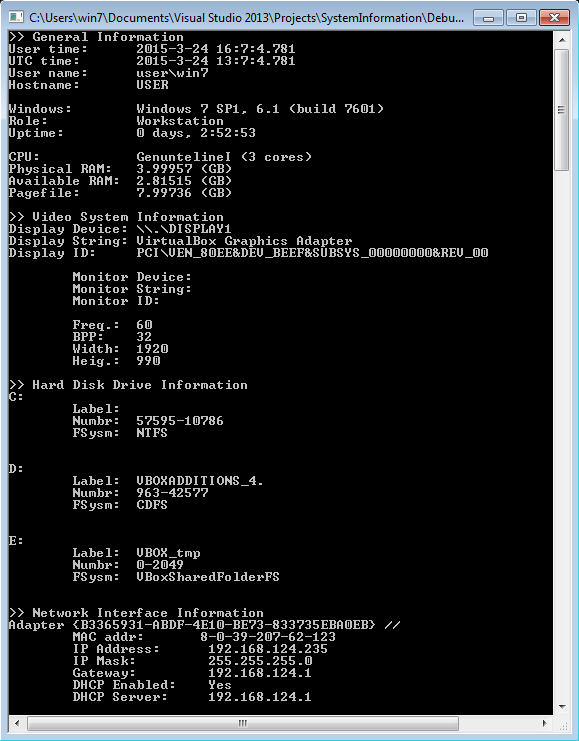
\includegraphics[scale=1]{res/results}
\caption{Результаты работы программы SystemInformation}
\end{figure}

Разница между локальным временем и UTC соответствует Московскому часовому поясу.

\begin{figure}[h!]
\centering
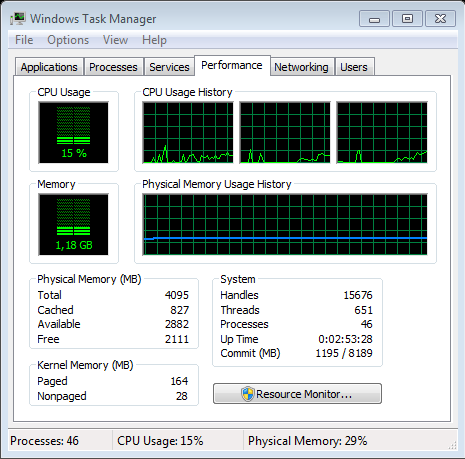
\includegraphics[scale=0.9]{res/taskmanager}
\caption{Диспетчер задач}
\end{figure}

\begin{figure}[h!]
\centering
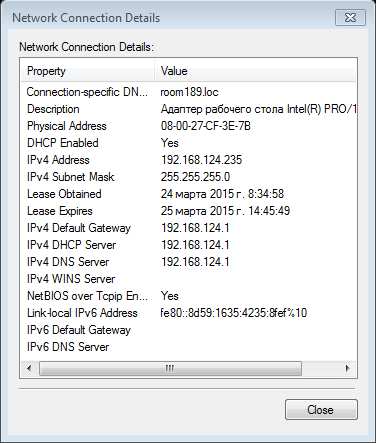
\includegraphics[scale=0.9]{res/network}
\caption{Информация о сетевом подключении}
\end{figure}

\begin{figure}[h!]
\centering
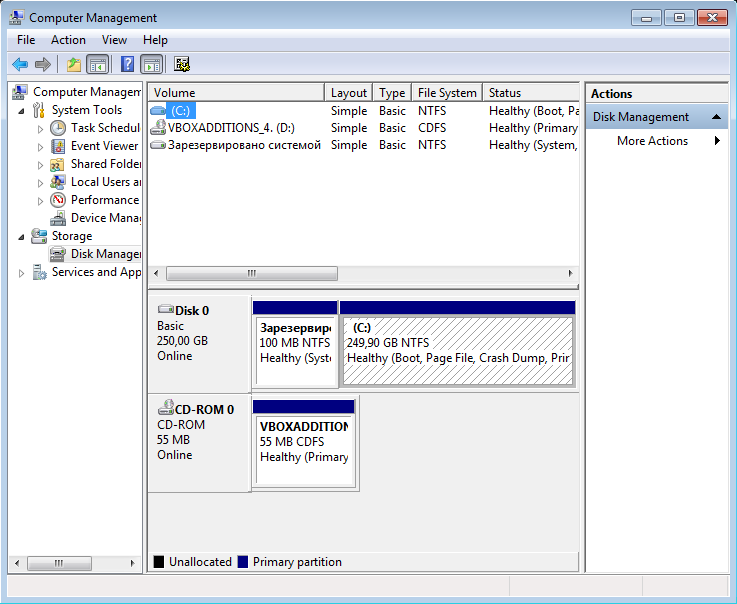
\includegraphics[scale=0.9]{res/disks}
\caption{Оснастка управления дисками}
\end{figure}

\section*{Листинг}
\addcontentsline{toc}{section}{Листинг}
Листинг 2 содержит исходный код программы SystemInformation. Как можно видеть, программа занимается только выводом информации, полученной от класса MySystem.

\lstinputlisting[language=C++, caption={Исходный код программы SystemInformation}]
{../../SystemInformation/SystemInformation/main.cpp}

%------------------------------------------------
\chapter*{Заключение}
\addcontentsline{toc}{chapter}{Заключение}

\vspace{1em}

В данной работе были рассмотрены основные механизмы сбора системной информации в ОС Windows.
\vspace{1em}

В отличии от мира linux, сбор системной информации осложнён разнообразностью форм её представления и разбросанностью по всей ОС.
\vspace{1em}

Разработанная программа позволяет получить следующую информацию:
\begin{enumerate}
\item время пользователя и UTC время;
\item имя пользователя и имя хоста;
\item версию операционной системы, с точностью до номера сервиспака и сборки;
\item производителя центрального процессора и доступных ядрах;
\item различные параметры оперативной памяти (как физической так и файла подкачки);
\item параметры работы видеосистемы;
\item локальные файловые накопители и используемые файловые системы;
\item параметры работы сетевой системы.
\end{enumerate}
\vspace{1em}

Корректность работы программы была проверена путём сверки данных с другими системными источниками. Данный код можно использовать в качестве динамической библиотеки в других, более масштабных проектах.


\end{document}
